\documentclass[12pt]{beamer}
\usepackage[utf8]{inputenc}
\usepackage[english]{babel}
\usepackage{tikz}
\usepackage{amssymb,amsmath}
\usepackage{hyperref}

\usetheme{Warsaw}

\usetikzlibrary{positioning,shapes,shadows,arrows}
\tikzstyle{myarrow}=[<-, >=open triangle 90, thick]
\tikzstyle{line}=[-, thick]

\begin{document}
	
	\author[Dimo]{
		\begin{table}[]
			\begin{tabular}{rl}
				\normalsize{Author:    } & \normalsize{Dimo Chanev} \\
				\scriptsize{Supervisiors:     } & \scriptsize{Doychin Boyadzhiev} \\
												& \scriptsize{Emil Kelevedjiev}
			\end{tabular}
		\end{table}
	}
	\title[Linear solver with infinity numbers (Linsol)]{\textbf{Linear solver with infinity numbers (Linsol)}}
	
	\begin{frame}
		\titlepage
	\end{frame}

	\begin{frame}
		\frametitle{Introduction}
		\begin{center}
			\Huge{$$\infty$$}
		\end{center}
		\begin{block}{}
			The project is separated in two parts:
            \begin{itemize}
            \item Infinity numbers
            \item Linsol (linear solver $\to$ simplex)
            \end{itemize}
		\end{block}
		\vspace{0.1cm}
		\begin{center}
			
\includegraphics[scale=0.1]{rust.png}
		\end{center}
		\vspace{1.1cm}
	\end{frame}

	\begin{frame}
		\frametitle{Infinity numbers}
		\begin{block}{Definition}
			Infinity number is a pair of real numbers. The one if for the real part and the other is for the infinity part.
			$$ (a; b) = a + b\infty, where\ a \in \mathbb{R}, b \in \{-1, 0, 1\}$$
		\end{block}
	\end{frame}

	\begin{frame}
		\frametitle{Infinity numbers}
		\begin{block}{Comparison}
			\begin{itemize}
				\item If the infinity part of the number is $>1$ the number is $=\infty$
				\item If the infinity part of the number is $>-1$ the number is $=-\infty$
				\item $\infty = \infty$ and $-\infty = -\infty$
				\item If the infinity parts of the both numbers are =0 then we compare the real parts as normal $\mathbb{R}$
			\end{itemize}
			\small{\textit{Note:} If the $infinity\ part\ of\ the\ number \notin \{-1, 0, 1\}$ we get it to one of these values}
		\end{block}
	\end{frame}

	\begin{frame}
		\frametitle{Infinity numbers}
		\begin{block}{Math operations}
			$$ (a; b) \pm (c; d) = (a \pm c; b \pm d)$$
			$$ (a; b) \times (c; d) = (ac; ad + bc + bd)$$
			\[ \frac{ (a; b)}{ (c; d)} = 
				\begin{cases}
					 (\frac{b}{d}; 0)           & d \neq 0\\
					 (\frac{a}{c}; \frac{b}{c}) & d = 0
				\end{cases} 
            \]   
			\small{\textit{Note:} If the $infinity\ part\ of\ the\ number \notin \{-1, 0, 1\}$ we get it to one of these values}
		\end{block}
	\end{frame}

	\begin{frame}
		\frametitle{Simplex}
		\begin{columns}
			\begin{column}{0.5\textwidth}
				\begin{block}{Definition}
					The simplex method is an algorithm for finding minimum/maximum value of a linear function with given linear constraints.
				\end{block}
				\begin{itemize}
					\item Finds the figure of interection of the graphics of the constraints.
					\item Loop all of the vertices and find where the target function's value is optimal
				\end{itemize}
			\end{column}
			\begin{column}{0.5\textwidth}
				\definecolor{qqqqff}{rgb}{0.,0.,1.}
				\definecolor{zzttqq}{rgb}{0.6,0.2,0.}
				\definecolor{uuuuuu}{rgb}{0.26666666666666666,0.26666666666666666,0.26666666666666666}
				\definecolor{cqcqcq}{rgb}{0.7529411764705882,0.7529411764705882,0.7529411764705882}
				\begin{tikzpicture}[line cap=round,line join=round,>=triangle 45,x=0.6cm,y=0.6cm]
					\draw [color=cqcqcq,, xstep=1.2cm,ystep=1.2cm] (0.,-4.) grid (6.,6.);
					\draw[->,color=black] (0.,0.) -- (6.,0.);
					\foreach \x in {,2.,4.}
					\draw[shift={ (\x,0)},color=black] (0pt,2pt) -- (0pt,-2pt) node[below] {\footnotesize $\x$};
					\draw[->,color=black] (0.,-4.) -- (0.,6.);
					\foreach \y in {-4.,-2.,2.,4.}
					\draw[shift={ (0,\y)},color=black] (2pt,0pt) -- (-2pt,0pt) node[left] {\footnotesize $\y$};
					\draw[color=black] (0pt,-10pt) node[right] {\footnotesize $0$};
					\clip (0.,-4.) rectangle (6.,6.);
					\fill[line width=1.2pt,color=zzttqq,fill=zzttqq,fill opacity=0.10000000149011612] (0.5,-0.5) -- (3.,-3.) -- (5.,-1.) -- (2.5,1.5) -- cycle;
					\draw [line width=1.2pt,domain=0.:6.] plot (\x,{ (--4.-1.*\x)/1.});
					\draw [line width=1.2pt,domain=0.:6.] plot (\x,{ (--1.-1.*\x)/-1.});
					\draw [line width=1.2pt,domain=0.:6.] plot (\x,{ (--6.-1.*\x)/-1.});
					\draw [line width=1.2pt,domain=0.:6.] plot (\x,{ (-0.-1.*\x)/1.});
					\draw [line width=1.2pt,color=zzttqq] (0.5,-0.5)-- (3.,-3.);
					\draw [line width=1.2pt,color=zzttqq] (3.,-3.)-- (5.,-1.);
					\draw [line width=1.2pt,color=zzttqq] (5.,-1.)-- (2.5,1.5);
					\draw [line width=1.2pt,color=zzttqq] (2.5,1.5)-- (0.5,-0.5);
					\draw [line width=1.2pt,domain=0.:6.] plot (\x,{ (-14.003262108984158--10.726297038005976*\x)/9.713927429924514});
					\begin{scriptsize}
					\draw[color=black] (-2.2446432797621805,6.516398410386435) node {$ $};
					\draw[color=black] (-3.0159725049671047,-3.462673440702271) node {$ $};
					\draw[color=black] (-1.352793863118987,-7.4639437964528135) node {$ $};
					\draw[color=black] (-3.0159725049671047,2.707960360937122) node {$ $};
					\draw [fill=uuuuuu] (0.5,-0.5) circle (2.0pt);
					\draw[color=uuuuuu] (0.5996332381809774,-0.11221211871838155) node {$ $};
					\draw [fill=uuuuuu] (3.,-3.) circle (2.0pt);
					\draw[color=uuuuuu] (3.1064532200969808,-2.5949280623467312) node {$ $};
					\draw [fill=uuuuuu] (5.,-1.) circle (2.0pt);
					\draw[color=uuuuuu] (5.1070883979722534,-0.5942928844714591) node {$ $};
					\draw [fill=uuuuuu] (2.5,1.5) circle (2.0pt);
					\draw[color=uuuuuu] (2.6002684160562493,1.8884230591568905) node {$ $};
					\draw[color=zzttqq] (1.467378616536517,-1.7994947988541532) node {$ $};
					\draw[color=zzttqq] (4.263447057904367,-2.064639220018346) node {$ $};
					\draw[color=zzttqq] (4.0224066750278284,0.7314292213495042) node {$ $};
					\draw[color=zzttqq] (1.2263382336599782,0.9965736425136968) node {$ $};
					\draw [fill=qqqqff] (-2.36516347120045,-4.0532223787497905) circle (2.0pt);
					\draw[color=qqqqff] (-2.2687473180498343,-3.6555057470035015) node {$ $};
					\draw [fill=qqqqff] (7.3487639587240645,6.673074659256185) circle (2.0pt);
					\draw[color=qqqqff] (7.44518011187468,6.347670142372858) node {$ $};
					\draw[color=black] (6.746163001532718,6.516398410386435) node {$ $};
					\end{scriptsize}
				\end{tikzpicture}
			\end{column}
		\end{columns}
	\end{frame}

	\begin{frame}
		\frametitle{Linsol}
		\textbf{Linsol} is a library written in Rust, which implements the simplex algorithm.\\
		\begin{center}
			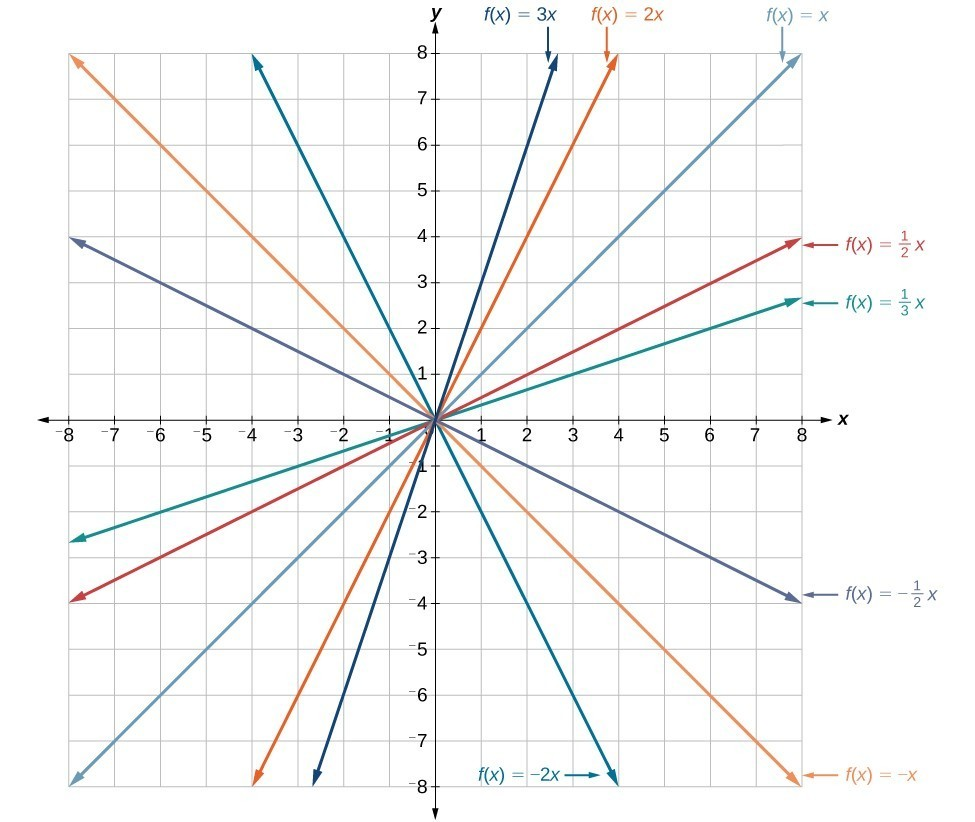
\includegraphics[scale=0.2]{graphs}
		\end{center}
	\end{frame}

	\begin{frame}
		\frametitle{Live Demo}
		
\includegraphics[scale=0.47]{demo}\\
		\small{Code: \href{https://github.com/Ro6afF/linsol}{https://github.com/Ro6afF/linsol}}
	\end{frame}

	\begin{frame}
		\frametitle{Future}
		\begin{itemize}
			\item Clarify the conception of the infinity numbers
			\item Make the code working
			\item Improve the memory consumption
			\item Improve the speed
			\item Implement integer solving
		\end{itemize}
		\begin{center}
			
\includegraphics[scale=0.15]{CodeYourFuture}
		\end{center}
		\vspace{-1cm}
	\end{frame}

	\begin{frame}
		\frametitle{Acknowledges}
		Special thanks for:
		\begin{itemize}
			\item Doychin Boyadzhiev
			\item Emil Kelevedjiev
		\end{itemize}
		\vspace{0.5cm}
		Acknowledges for:
		\begin{itemize}
			\item \href{http://www.math.bas.bg/omi/hssimi/}{High School Students Institute of Mathematics and Informatics}
			\item \href{http://www.math.bas.bg/}{Bulgarian Academy of Sciences}
			\item \href{http://www.smg.bg}{Sofia High School of Mathematics}
		\end{itemize}
	\end{frame}
	
	\begin{frame}
	\frametitle{Resources}
		\begin{itemize}
			\item%{rust}
			{\itshape Rust compiler toolchain:}
			\texttt{https://www.rust-lang.org}. \\
            Copyright \copyright\ 2015 The Rust Project Developers
			\item%{latex}
			{\itshape \LaTeX}.
			\texttt{https://www.latex-project.org/}.
		\end{itemize}
	\end{frame}
	
	\begin{frame}
	\begin{center}
	{\Huge Questions}
    
\includegraphics[scale=0.3]{quest}
	\end{center}
	\end{frame}
	
	\begin{frame}
		\begin{center}
		
\includegraphics{thx}
		\end{center}
	\end{frame}

\end{document}
